\graphicspath{ {./images/4_Analyte_curation} }
\newpage

\section{Analyte curation}
The purpose of analyte curation is to decide which analytes can be measured at sufficient quality in the data set, thus improving the overall quality and reliability of the data.
There are four methods that can be used to perform analyte curation, as discussed below. 

\subsection{Based on percentages of passing spectra}
Analytes are curated based on the quality criteria that were chosen in the \menu{Spectra curation} tab.
An analyte passes curation if it meets the quality criteria in a percentage of spectra exceeding a chosen cut-off percentage.
The analyte is then used for total area normalization in all samples. 
The cut-off percentage can be set for each glycosylation site individually, or one cut-off can be applied to all of them.

There is an option to specify biological groups in the data. 
When used, an analyte that fulfills the quality criteria in a percentage exceeding the cut-off for at least one of the biological groups passes curation.
It will then be used for total area normalization in all samples, irrespective of their biological groups.
It is possible to ignore certain biological groups from this assessment (e.g., when dealing with a small number of samples in one of the groups).

Optionally, select sample types to ignore during the assessment, such as blanks and standards.
When curating per biological group, samples types that are not assigned to a biological groups are automatically excluded, even when they are not explicitly selected here.

\begin{optionalbox}
	If the data contains total and specific immunoglobulins, there is an option to exclude either one as a sample types during analyte curation.
	It is recommended to exclude total samples and base the curation solely on the specific samples.
\end{optionalbox}

One or two QC parameters may be excluded from the assessment entirely via the gears icon in the top-right corner of the \textsf{Method for analyte curation} box.

After performing curation, an interactive plot is generated for each glycosylation site.
Each analyte and charge state is represented by a bar in the plot, color-coded to indicate whether it passed curation.
If curation was performed per biological group, the plots are made for each group.

\begin{center}
	
\includegraphics[scale=0.55]{curation_results.png}
\end{center}


\newpage
Below the bar plots, a table listing all analytes is generated.
For each charge state, the table indicates whether the analyte passed curation, and there is a checkbox to include or exclude that analyte from further analysis.

Manual inclusion or exclusion of analytes should only be done when external information warrants this.

\begin{optionalbox}
	There is a toggle option to automatically include all charge states of analyte if at least one of the charge states passes curation.
	When using this option, strong interferences should be excluded (e.g., by manual inspection of raw data or LaCyTools/SweetSuite/Skyline output).
	Then, this likely increases accuracy at the expense of precision.
\end{optionalbox}


\subsection{Based on average QC parameters}
When the average values of the QC parameters fulfill the chosen requirements, then that analyte passes curation and is used for further analysis in all samples.
Average QC values can be calculated as either the mean or median.
An acceptable range must be set for the average mass accuracy.
For SweetSuite or LaCyTools data, a maximum value for the average IPQ and a minimum value for the $S/N$ must be specified.
For Skyline data, a minimum average IDP value and minimum average total area must be specified.

Like when curating based on the percentages of passing spectra, curation can be performed per biological group, and it is possible to exclude sample types from the assessment.

The curation results are visualized for each glycosylation site in a binary heatmap, with charge states on the $y$-axis and analytes on the $x$-axis.
The tiles are color-coded based on whether an analyte passed curation.
When hovering over the tiles, the average values for the QC parameters are displayed.

Below the heatmaps, the same checkbox table is generated as when performing curation based on the percentages of passing spectra. 

\begin{center}
	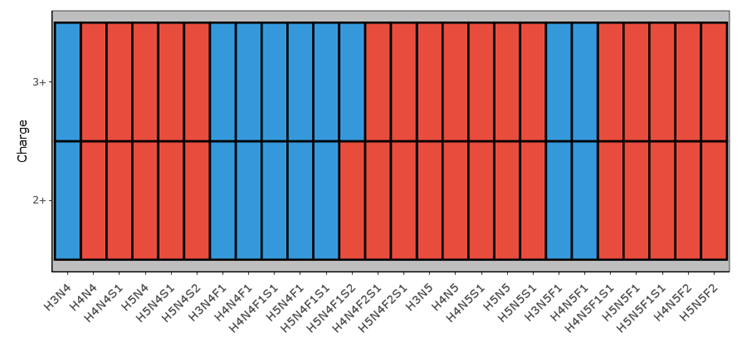
\includegraphics[scale=0.75]{heatmap.png}
\end{center}



\newpage

\subsection{Per sample}
If an analyte meets the quality criteria in one sample, it is used for total area normalization in that sample. 
If the same analyte does not meet the criteria in some other sample, then it is not used for normalization in that particular sample.
The results from this curation method are not visualized, but a table containing checkboxes is again generated.

\subsection{Supply an analyte list}
\emph{This method should only be used if you performed analyte curation based on your data outside of GlycoDash.}

You can choose to supply an analyte list (as a \texttt{.xlsx} file or R object) that contains the names of all analytes that should be kept. 
This method does not distinguish between charge states: all charge states of the specified analytes will pass the curation.



